\documentclass[12pt,a4paper]{article}

% --- Page Layout -------------------------------------------------------------
\usepackage[a4paper, margin=0.8in, headheight=14pt]{geometry}

% --- Fonts (XeLaTeX) ---------------------------------------------------------
\usepackage{fontspec}
\usepackage{unicode-math}
\setmainfont{TeX Gyre Pagella}
\setmonofont[Scale=0.88]{TeX Gyre Cursor}
\setmathfont{Latin Modern Math}

% --- Packages ---------------------------------------------------------------
\usepackage{xcolor}
\usepackage{titlesec}
\usepackage{enumitem}
\usepackage{tabularx}
\usepackage{booktabs}
\usepackage{array}
\usepackage{amsmath}
\usepackage{tikz}
\usetikzlibrary{shapes.geometric, arrows.meta, positioning, calc, fit, decorations.pathreplacing}
\usepackage{tcolorbox}
\tcbuselibrary{skins, breakable}
\usepackage{hyperref}
\usepackage{fancyhdr}
\usepackage{graphicx}
\usepackage{microtype}
\hyphenpenalty=10000
\exhyphenpenalty=10000
\sloppy
\usepackage{caption}
\usepackage{setspace}
\usepackage{multirow}
\usepackage{tocloft}

% --- Q&A helper --------------------------------------------------------------
\newcommand{\Q}[1]{\textbf{#1}\par\noindent\ignorespaces}

% --- Colour Palette ----------------------------------------------------------
\definecolor{myred}{RGB}{196,30,58}
\definecolor{mydark}{RGB}{30,30,50}
\definecolor{mygreen}{RGB}{14,120,80}
\definecolor{myteal}{RGB}{0,130,140}
\definecolor{myamber}{RGB}{180,100,0}
\definecolor{mypurple}{RGB}{100,30,160}
\definecolor{mygray}{RGB}{246,247,249}
\definecolor{mgframe}{RGB}{180,185,200}
\definecolor{watermark}{RGB}{145,150,170}
\definecolor{hdrred}{RGB}{250,232,235}
\definecolor{hdrgreen}{RGB}{220,244,233}
\definecolor{hdrteal}{RGB}{220,242,244}
\definecolor{hdramber}{RGB}{253,242,215}
\definecolor{hdrpurple}{RGB}{238,228,255}
\definecolor{hdrgray}{RGB}{238,240,245}
\definecolor{rowalt}{RGB}{250,251,253}

% --- Section Formatting ------------------------------------------------------
\titleformat{\section}
  {\large\bfseries\color{myred}}{\thesection.}{0.5em}{}
  [\vspace{1pt}{\color{myred}\rule{\linewidth}{0.8pt}}]
\titleformat{\subsection}
  {\normalsize\bfseries\color{myteal}}{\thesubsection}{0.5em}{}
\titlespacing*{\section}{0pt}{18pt}{7pt}
\titlespacing*{\subsection}{0pt}{11pt}{4pt}

% --- Paragraph ---------------------------------------------------------------
\setlength{\parindent}{0pt}
\setlength{\parskip}{4pt}

% --- TOC Styling -------------------------------------------------------------
\renewcommand{\cfttoctitlefont}{\large\bfseries\color{myred}}
\renewcommand{\cftaftertoctitle}{\par\noindent{\color{myred}\rule{\linewidth}{0.8pt}}}
\setlength{\cftbeforetoctitleskip}{0pt}
\setlength{\cftaftertoctitleskip}{6pt}
\renewcommand{\cftsecfont}{\normalsize\bfseries\color{mydark}}
\renewcommand{\cftsecpagefont}{\normalsize\bfseries\color{mydark}}
\renewcommand{\cftsecleader}{\cftdotfill{\cftdotsep}}
\setlength{\cftbeforesecskip}{7pt}
\renewcommand{\cftsubsecfont}{\small\color{mydark}}
\renewcommand{\cftsubsecpagefont}{\small\color{mydark}}
\setlength{\cftbeforesubsecskip}{3pt}
\setlength{\cftsubsecindent}{1.4em}

% --- Table helpers -----------------------------------------------------------
\renewcommand{\arraystretch}{1.45}
\setlength{\tabcolsep}{6pt}
\newcolumntype{B}[1]{>{\small\bfseries\raggedright\arraybackslash}m{#1}}
\newcolumntype{Y}{>{\small\raggedright\arraybackslash}X}
\renewcommand{\tabularxcolumn}[1]{m{#1}}

% --- Header / Footer ---------------------------------------------------------
\pagestyle{fancy}
\fancyhf{}
\fancyhead[L]{\small\color{myred}\textbf{BS-CH101}\;\color{mydark}--- Chemistry-I}
\fancyhead[R]{\small\color{myteal}\textbf{Module 3 Notes}}
\fancyfoot[C]{\small\color{mydark}\thepage}
\fancyfoot[R]{\small\color{watermark}\textit{\copyright\ Biraj}}
\renewcommand{\headrulewidth}{0.5pt}
\renewcommand{\footrulewidth}{0.3pt}

% --- Hyperref ---------------------------------------------------------------
\hypersetup{
  colorlinks=true, linkcolor=myteal, urlcolor=myteal,
  pdfauthor={Biraj Sarkar},
  pdftitle={BS-CH101 --- Module 3 Notes}
}

% --- tcolorbox styles --------------------------------------------------------
\tcbset{
  tikzbox/.style={
    colback=mygray, colframe=mgframe, boxrule=0.6pt, arc=4pt,
    left=8pt, right=8pt, top=6pt, bottom=6pt,
    colbacktitle=mgframe, coltitle=mydark,
    fonttitle=\small\bfseries
  },
  defbox/.style={
    colback=hdrgreen, colframe=mygreen, boxrule=0.8pt, arc=4pt,
    left=9pt, right=9pt, top=6pt, bottom=6pt,
    colbacktitle=mygreen, coltitle=white,
    fonttitle=\small\bfseries
  },
  formulabox/.style={
    colback=hdrteal, colframe=myteal, boxrule=0.8pt, arc=4pt,
    left=9pt, right=9pt, top=7pt, bottom=7pt,
    colbacktitle=myteal, coltitle=white,
    fonttitle=\small\bfseries
  },
  examplebox/.style={
    colback=hdramber, colframe=myamber, boxrule=0.8pt, arc=4pt,
    left=9pt, right=9pt, top=6pt, bottom=6pt,
    colbacktitle=myamber, coltitle=white,
    fonttitle=\small\bfseries
  },
  masonbox/.style={
    colback=hdrpurple, colframe=mypurple, boxrule=0.8pt, arc=4pt,
    left=9pt, right=9pt, top=6pt, bottom=6pt,
    colbacktitle=mypurple, coltitle=white,
    fonttitle=\small\bfseries
  },
  exambox/.style={
    colback=hdrpurple, colframe=mypurple, boxrule=1pt, arc=5pt,
    left=10pt, right=10pt, top=8pt, bottom=8pt,
    colbacktitle=mypurple, coltitle=white,
    fonttitle=\bfseries,
    breakable, title after break={\textbf{Frequently Asked / Viva Questions (contd.)}}}
}
\tcbset{breakable}

% --- TikZ styles -------------------------------------------------------------
\tikzset{
  block/.style={rectangle, draw=myteal, fill=hdrteal,
    text width=2.4cm, align=center, minimum height=0.95cm,
    font=\small, rounded corners=3pt, line width=0.7pt},
  redblock/.style={rectangle, draw=myred, fill=hdrred,
    text width=2.4cm, align=center, minimum height=0.95cm,
    font=\small, rounded corners=3pt, line width=0.7pt},
  netnode/.style={rectangle, draw=myteal, fill=hdrteal,
    text width=1.5cm, align=center, minimum height=0.8cm,
    font=\small, rounded corners=3pt, line width=0.7pt},
  sumjunc/.style={circle, draw=myamber, fill=hdramber,
    minimum size=0.62cm, font=\small, line width=0.8pt},
  snode/.style={circle, draw=mypurple, fill=hdrpurple,
    minimum size=0.55cm, font=\footnotesize, line width=0.7pt},
  arrow/.style={-Stealth, thick, color=mydark},
  redarrow/.style={-Stealth, thick, color=myred},
  line/.style={thick, color=mydark}
}

\begin{document}

\begin{center}
  {\LARGE\bfseries\color{myred} BS-CH101 / BS-CH201 --- Chemistry-I}\\[5pt]
  {\normalsize\color{mydark} Semester I \quad$\bullet$\quad 3L:1T:0P \quad$\bullet$\quad 4 Credits}\\[3pt]
  {\normalsize\color{myteal}\textbf{Module 3 Exam Notes: Intermolecular Forces and Potential Energy Surfaces}}\\[3pt]
  {\small\color{mydark} CGEC \;$|$\; B.Tech ECE (2023--27) \;$|$\; \textit{Biraj Sarkar}}
\end{center}
\vspace{2pt}
\noindent{\color{myred}\rule{\linewidth}{1.5pt}}
\vspace{2pt}

\hypersetup{linkcolor=mydark}
\tableofcontents
\hypersetup{linkcolor=myteal}
\newpage
% ===============================================================================
\section{Intermolecular Forces and Potential Energy Surfaces}
% ===============================================================================

\begin{tcolorbox}[defbox]
\textbf{Intermolecular forces} are attractive or repulsive forces between molecules or ions. They are weaker than covalent bonds but strongly affect boiling point, solubility, viscosity, and real-gas behaviour.
\end{tcolorbox}

\subsection{Ionic, Dipole and Van der Waals Interactions}
Ionic interactions are strongest among common non-covalent interactions. Dipole-dipole forces occur between polar molecules. London dispersion forces arise from temporary induced dipoles and exist in all molecules.

\begin{tabularx}{\linewidth}{|B{3.2cm}|Y|Y|}
\hline
\textbf{Interaction} & \textbf{Origin} & \textbf{Example} \\
\hline
Ion-ion & Attraction between full charges & $\mathrm{Na^+}$ and $\mathrm{Cl^-}$ \\
\hline
Ion-dipole & Ion attracts polar molecule & Hydration of $\mathrm{Na^+}$ \\
\hline
Dipole-dipole & Permanent dipoles align & $\mathrm{HCl}$ molecules \\
\hline
London dispersion & Instantaneous induced dipoles & Noble gases, hydrocarbons \\
\hline
Hydrogen bonding & H attached to F, O, or N interacts with lone pair & Water, alcohols \\
\hline
\end{tabularx}

\subsection{Potential Energy Curve}
The potential energy between two particles depends on separation distance. At equilibrium distance $r_e$, attractive and repulsive forces balance and potential energy is minimum.

\begin{tcolorbox}[tikzbox, title={Potential Energy Curve for Intermolecular Interaction}]
\centering
\begin{tikzpicture}[scale=0.92]
  \draw[->, thick] (0,0) -- (7.2,0) node[right] {$r$};
  \draw[->, thick] (0,-2.2) -- (0,2.2) node[above] {$V(r)$};
  \draw[myteal, thick, domain=0.45:6.7, samples=160]
    plot(\x,{1.8*exp(-2.2*\x)-2.4*\x*exp(-1.05*\x)});
  \draw[dashed] (1.32,0) -- (1.32,-1.55);
  \node[font=\small] at (1.32,0.35) {$r_e$};
  \node[font=\small] at (4.6,-1.0) {attraction};
  \node[font=\small] at (1.0,1.5) {repulsion};
\end{tikzpicture}
\end{tcolorbox}

\subsection{Equations of State for Real Gases}
Ideal gas equation assumes no intermolecular force and zero molecular volume. Real gases deviate at high pressure and low temperature.

\begin{tcolorbox}[formulabox, title={Van der Waals Equation}]
\[
\left(P+\frac{a n^2}{V^2}\right)(V-nb)=nRT
\]
where $a$ corrects attractive forces and $b$ corrects finite molecular volume.
\end{tcolorbox}

\subsection{Critical Phenomena}
The critical temperature $T_c$ is the temperature above which a gas cannot be liquefied by pressure alone. At the critical point, liquid and vapour become indistinguishable.

\begin{tcolorbox}[formulabox, title={Critical Constants for a Van der Waals Gas}]
\[
V_c=3nb,\qquad P_c=\frac{a}{27b^2},\qquad T_c=\frac{8a}{27Rb}
\]
\end{tcolorbox}

\begin{tcolorbox}[exambox, title={Exam Points}]
\begin{itemize}[leftmargin=*, itemsep=2pt, topsep=2pt]
  \item Compare intermolecular forces by strength and origin.
  \item Draw the potential energy curve and mark $r_e$ and minimum energy.
  \item For real gases, explain physical meaning of constants $a$ and $b$.
  \item Define critical temperature, pressure, and volume clearly.
\end{itemize}
\end{tcolorbox}

% ===============================================================================
\section{Detailed Notes on Forces, Real Gases and Critical Behaviour}
% ===============================================================================

\subsection{Origin and Strength of Intermolecular Forces}
Intermolecular force strength depends on charge, polarity, polarizability, and molecular shape. Ionic interactions are strong because full charges are involved. Dispersion forces are weak individually but become important for large molecules with many electrons.

\begin{tabularx}{\linewidth}{|B{3.4cm}|Y|Y|}
\hline
\textbf{Force} & \textbf{Approximate strength trend} & \textbf{Property affected} \\
\hline
Ion-ion & Very strong & Melting point of ionic solids \\
\hline
Ion-dipole & Strong & Hydration and solubility of salts \\
\hline
Hydrogen bond & Moderate to strong & Boiling point of water and alcohols \\
\hline
Dipole-dipole & Moderate & Boiling point of polar molecules \\
\hline
London dispersion & Weak to moderate & Liquefaction of non-polar gases \\
\hline
\end{tabularx}

\subsection{Potential Energy and Force Relation}
The force between two particles is related to the potential energy curve by:
\[
F=-\frac{dV}{dr}
\]
At the equilibrium separation $r_e$, potential energy is minimum, so:
\[
\left(\frac{dV}{dr}\right)_{r=r_e}=0,\qquad F=0
\]
For $r<r_e$, repulsive force dominates. For $r>r_e$, attractive force dominates.

\begin{tcolorbox}[examplebox, title={Exam Interpretation of Potential Energy Curve}]
If two molecules are very far apart, $V(r)\approx0$. As they approach, attraction lowers the potential energy. At $r_e$, the most stable separation is reached. If they come closer than $r_e$, electron-cloud repulsion sharply increases energy.
\end{tcolorbox}

\subsection{Lennard-Jones Potential}
A common model for non-bonded interaction is:
\[
V(r)=4\varepsilon\left[\left(\frac{\sigma}{r}\right)^{12}-\left(\frac{\sigma}{r}\right)^6\right]
\]
The $r^{-12}$ term represents short-range repulsion and the $r^{-6}$ term represents London attraction. $\varepsilon$ indicates well depth, i.e. strength of attraction.

\begin{tabularx}{\linewidth}{|B{3cm}|Y|}
\hline
\textbf{Term} & \textbf{Physical meaning} \\
\hline
$\left(\sigma/r\right)^{12}$ & Repulsion due to electron-cloud overlap \\
\hline
$-\left(\sigma/r\right)^6$ & Attractive dispersion interaction \\
\hline
$\varepsilon$ & Depth of potential well; higher value means stronger attraction \\
\hline
$r_e$ & Separation at minimum potential energy \\
\hline
\end{tabularx}

\subsection{Compressibility Factor and Deviation from Ideality}
Deviation from ideal gas behaviour is often measured using compressibility factor:
\[
Z=\frac{PV}{nRT}
\]
For an ideal gas, $Z=1$. For a real gas, $Z<1$ indicates attraction-dominated behaviour and $Z>1$ indicates repulsion or finite-volume dominated behaviour.

\begin{tcolorbox}[tikzbox, title={Compressibility Factor: Qualitative Behaviour}]
\centering
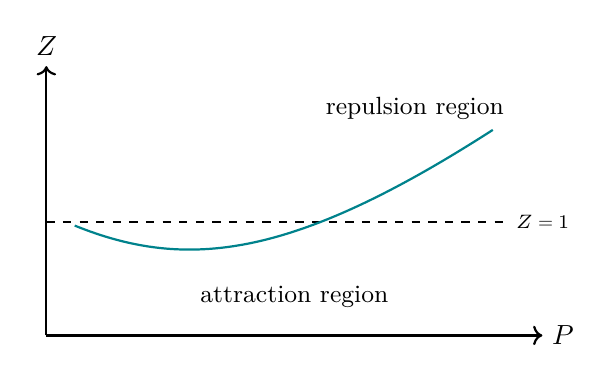
\begin{tikzpicture}[scale=0.9]
  \draw[->, thick] (0,0) -- (7,0) node[right] {$P$};
  \draw[->, thick] (0,0) -- (0,3.8) node[above] {$Z$};
  \draw[dashed] (0,1.6) -- (6.5,1.6) node[right,font=\scriptsize] {$Z=1$};
  \draw[myteal, thick] (0.4,1.55) .. controls (2,0.9) and (3.5,1.1) .. (6.3,2.9);
  \node[font=\small] at (3.5,0.55) {attraction region};
  \node[font=\small] at (5.2,3.2) {repulsion region};
\end{tikzpicture}
\end{tcolorbox}

\subsection{Critical Constants from Van der Waals Equation}
For one mole:
\[
\left(P+\frac{a}{V_m^2}\right)(V_m-b)=RT
\]
At the critical point, the isotherm has a point of inflection:
\[
\left(\frac{\partial P}{\partial V_m}\right)_T=0,\qquad
\left(\frac{\partial^2 P}{\partial V_m^2}\right)_T=0
\]
Solving these conditions gives:
\[
V_c=3b,\qquad P_c=\frac{a}{27b^2},\qquad T_c=\frac{8a}{27Rb}
\]
These relations are often asked as short derivation or formula-based questions.

\begin{tcolorbox}[examplebox, title={Solved Example: Critical Volume}]
If van der Waals constant $b=0.040\ \mathrm{L\,mol^{-1}}$, then:
\[
V_c=3b=3(0.040)=0.120\ \mathrm{L\,mol^{-1}}
\]
\end{tcolorbox}

\begin{tcolorbox}[masonbox, title={How to Score in This Module}]
\begin{itemize}[leftmargin=*, itemsep=2pt, topsep=2pt]
  \item Write force origin, example, and property affected for each intermolecular force.
  \item In potential energy questions, always mark attraction, repulsion, $r_e$, and energy minimum.
  \item For real gases, explain that $a$ corrects pressure and $b$ corrects volume.
  \item Use $Z=PV/nRT$ to discuss positive and negative deviation.
\end{itemize}
\end{tcolorbox}

\subsection{Hydrogen Bonding in Detail}
Hydrogen bonding occurs when hydrogen is covalently bonded to a highly electronegative atom such as F, O, or N and interacts with a lone pair on another electronegative atom.

\begin{tabularx}{\linewidth}{|B{3.3cm}|Y|Y|}
\hline
\textbf{Type} & \textbf{Meaning} & \textbf{Example} \\
\hline
Intermolecular hydrogen bonding & Hydrogen bond between different molecules & Water, alcohols, HF \\
\hline
Intramolecular hydrogen bonding & Hydrogen bond within the same molecule & o-nitrophenol type structures \\
\hline
Strong hydrogen bonding & Shorter and more directional interaction & HF, water network \\
\hline
Weak hydrogen bonding & Longer and less directional interaction & C--H based weak interactions \\
\hline
\end{tabularx}

\begin{tcolorbox}[examplebox, title={Exam Explanation: Boiling Point of Water}]
Water has a much higher boiling point than $\mathrm{H_2S}$ because oxygen is highly electronegative and forms extensive intermolecular hydrogen bonding. More heat is required to break this associated network before molecules escape into vapour phase.
\end{tcolorbox}

\subsection{Corresponding States and Reduced Variables}
The law of corresponding states states that gases behave similarly when compared at the same reduced temperature and reduced pressure.

\begin{tcolorbox}[formulabox, title={Reduced Variables}]
\[
T_r=\frac{T}{T_c},\qquad P_r=\frac{P}{P_c},\qquad V_r=\frac{V}{V_c}
\]
where $T_c$, $P_c$, and $V_c$ are critical constants.
\end{tcolorbox}

\subsection{Boyle Temperature}
At Boyle temperature, a real gas behaves nearly ideally over a considerable pressure range because attractive and repulsive deviations approximately cancel.
\[
Z\approx1
\]
For a van der Waals gas, the Boyle temperature is approximately:
\[
T_B=\frac{a}{Rb}
\]

\begin{tcolorbox}[examplebox, title={Solved Example: Boyle Temperature}]
If $a=1.36\ \mathrm{L^2\,atm\,mol^{-2}}$ and $b=0.0318\ \mathrm{L\,mol^{-1}}$:
\[
T_B=\frac{a}{Rb}=\frac{1.36}{(0.0821)(0.0318)}
\]
\[
T_B\approx521\ \mathrm{K}
\]
\end{tcolorbox}

\subsection{Joule-Thomson Effect}
When a real gas expands through a porous plug from high pressure to low pressure without external work and without heat exchange, its temperature may change. This is called Joule-Thomson effect.

\begin{tcolorbox}[defbox]
\textbf{Inversion temperature:} The temperature at which Joule-Thomson coefficient becomes zero. Below it, gas cools on expansion; above it, gas warms on expansion.
\end{tcolorbox}

\begin{tabularx}{\linewidth}{|B{3.0cm}|Y|Y|}
\hline
\textbf{Condition} & \textbf{Joule-Thomson coefficient} & \textbf{Observation} \\
\hline
$T<T_i$ & Positive & Gas cools on expansion \\
\hline
$T=T_i$ & Zero & No temperature change \\
\hline
$T>T_i$ & Negative & Gas warms on expansion \\
\hline
\end{tabularx}

\subsection{Potential Energy Surface in Chemical Reactions}
A potential energy surface shows how molecular energy changes with geometry. Reactants, products, intermediates, and transition states are represented as regions on the surface.

\begin{tcolorbox}[tikzbox, title={Reaction Path on a Potential Energy Surface}]
\centering
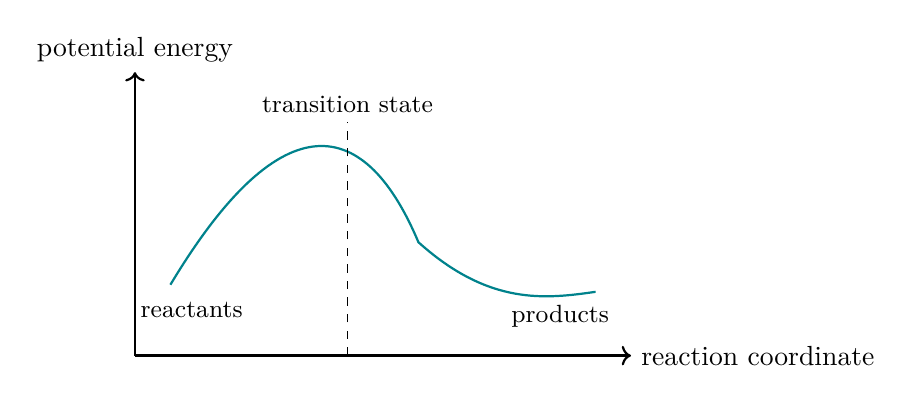
\begin{tikzpicture}[scale=0.9]
  \draw[->, thick] (0,0) -- (7,0) node[right] {reaction coordinate};
  \draw[->, thick] (0,0) -- (0,4) node[above] {potential energy};
  \draw[myteal, thick] (0.5,1.0) .. controls (2,3.5) and (3.2,3.5) .. (4.0,1.6)
    .. controls (5.0,0.7) and (5.8,0.8) .. (6.5,0.9);
  \node[font=\small] at (0.8,0.65) {reactants};
  \node[font=\small] at (3.0,3.55) {transition state};
  \node[font=\small] at (6.0,0.55) {products};
  \draw[dashed] (3.0,0) -- (3.0,3.3);
\end{tikzpicture}
\end{tcolorbox}

\begin{tcolorbox}[masonbox, title={Previous-Year Style Questions}]
\begin{enumerate}[leftmargin=*, itemsep=4pt, topsep=2pt]
  \item Compare ion-dipole, dipole-dipole, hydrogen bonding and dispersion forces.
  \item Explain the potential energy curve for two interacting molecules.
  \item Derive or state critical constants of a van der Waals gas.
  \item Explain compressibility factor and deviation from ideal behaviour.
  \item Write short notes on Joule-Thomson effect and inversion temperature.
\end{enumerate}
\end{tcolorbox}

\subsection{Applications of Intermolecular Forces in Engineering Chemistry}
Intermolecular forces are not only theoretical; they explain important material and chemical behaviour.

\begin{tabularx}{\linewidth}{|B{3.0cm}|Y|Y|}
\hline
\textbf{Application} & \textbf{Force involved} & \textbf{Importance} \\
\hline
Solubility of salts in water & Ion-dipole force & Hydration stabilizes ions in solution \\
\hline
Polymer strength & Dipole interaction and hydrogen bonding & Controls toughness, flexibility and melting range \\
\hline
Adsorption on catalyst & van der Waals and polar interactions & Reactants attach to active surface sites \\
\hline
Boiling point of liquids & Hydrogen bonding and dispersion & Stronger forces increase boiling point \\
\hline
Protein structure & Hydrogen bonding and hydrophobic interaction & Maintains secondary and tertiary structure \\
\hline
\end{tabularx}

\begin{tcolorbox}[examplebox, title={Exam Answer: Like Dissolves Like}]
Polar solvents dissolve ionic and polar solutes because ion-dipole or dipole-dipole interactions compensate for the energy needed to separate solute particles. Non-polar solutes dissolve better in non-polar solvents because dispersion forces are similar in both.
\end{tcolorbox}
\newpage
\begin{center}
  {\large\bfseries\color{myred} Quick Revision --- Module 3}\\[3pt]
  {\small\color{mydark} Intermolecular Forces and Potential Energy Surfaces $|$ BS-CH101}
\end{center}
\noindent{\color{myred}\rule{\linewidth}{1.2pt}}
\vspace{4pt}

\begin{tcolorbox}[formulabox, title={Key Formulas at a Glance}]
\begin{tabularx}{\linewidth}{|B{4.0cm}|Y|}
\hline
\textbf{Formula / Rule} & \textbf{Meaning} \\
\hline
$F=-\displaystyle\frac{dV}{dr}$ & Force is negative gradient of potential energy. \\
\hline
$PV=nRT$ & Ideal gas equation. \\
\hline
$\left(P+\displaystyle\frac{an^2}{V^2}\right)(V-nb)=nRT$ & Van der Waals real-gas equation. \\
\hline
$V_c=3nb$ & Critical volume for van der Waals gas. \\
\hline
$P_c=\displaystyle\frac{a}{27b^2}$ & Critical pressure for one mole form. \\
\hline
$T_c=\displaystyle\frac{8a}{27Rb}$ & Critical temperature for one mole form. \\
\hline
\end{tabularx}
\end{tcolorbox}

\begin{tcolorbox}[defbox, title={One-Line Definitions}]
\begin{itemize}[leftmargin=*, itemsep=2pt, topsep=2pt]
  \item \textbf{Intermolecular force:} Force acting between molecules or ions.
  \item \textbf{Dipole moment:} Product of charge and separation in a polar molecule.
  \item \textbf{Hydrogen bond:} Strong dipole interaction involving H bonded to F, O, or N.
  \item \textbf{Potential energy surface:} Energy variation with molecular geometry.
  \item \textbf{Real gas:} Gas that deviates from ideal behaviour due to volume and attraction.
  \item \textbf{Critical temperature:} Highest temperature at which gas can be liquefied by pressure.
\end{itemize}
\end{tcolorbox}

\begin{tcolorbox}[exambox, title={Frequently Asked / Viva Questions}]
\begin{enumerate}[topsep=0pt, label=\textbf{Q\arabic*.}, itemsep=5pt]
  \item \Q{What are intermolecular forces?}
    Forces of attraction or repulsion acting between separate molecules or ions.
  \item \Q{Arrange common forces in increasing strength.}
    London dispersion $<$ dipole-dipole $<$ hydrogen bonding $<$ ion-dipole $<$ ion-ion.
  \item \Q{Why does boiling point increase with stronger intermolecular force?}
    More energy is needed to separate molecules into vapour.
  \item \Q{What is equilibrium separation in a potential energy curve?}
    It is the distance where potential energy is minimum and net force is zero.
  \item \Q{What causes repulsion at very small distance?}
    Overlap of electron clouds and nuclear repulsion.
  \item \Q{Why do real gases deviate from ideal behaviour?}
    Molecules have finite volume and attractive forces.
  \item \Q{What is the role of $a$ in van der Waals equation?}
    It corrects pressure for intermolecular attraction.
  \item \Q{What is the role of $b$ in van der Waals equation?}
    It corrects volume for finite molecular size.
  \item \Q{Define critical point.}
    The point at which liquid and vapour phases become indistinguishable.
  \item \Q{What is critical temperature?}
    The highest temperature above which gas cannot be liquefied by pressure alone.
\end{enumerate}
\end{tcolorbox}

\begin{tcolorbox}[tikzbox, title={Summary Reference Table}]
\begin{tabularx}{\linewidth}{|B{3.2cm}|Y|Y|}
\hline
\textbf{Concept} & \textbf{Meaning} & \textbf{Must write in exam} \\
\hline
Intermolecular forces & Non-covalent forces between species & Strength order and examples \\
\hline
Potential curve & Energy versus separation & Minimum at $r_e$ \\
\hline
Real gas & Non-ideal gas & Van der Waals correction terms \\
\hline
Critical point & End point of liquid-vapour boundary & $T_c$, $P_c$, $V_c$ definitions \\
\hline
\end{tabularx}
\end{tcolorbox}

\end{document}
